\documentclass[11pt]{article}
\usepackage{tutorial-students}
\usepackage{tikz}
\usetikzlibrary{positioning, shapes.geometric, arrows.meta}
\usepackage{tkz-graph}

\newcommand{\fillinMCmath}[1]{
\begin{tikzpicture}\draw circle [radius=0.5em];\end{tikzpicture}\ #1}
\newcommand{\fillinMCmathsoln}[1]{
\begin{tikzpicture}\draw[black, fill=blue] circle [radius=0.5em];\end{tikzpicture}\ #1}

\newcommand{\opt}{\mbox{opt}}
\newcommand{\rank}{\mbox{rank}}
\newcommand{\finalmarks}{\mbox{marks}}
\newcommand{\solnn}{\mbox{soln}}
\newcommand{\true}{\mbox{True}}
\newcommand{\false}{\mbox{False}}


\author{}
\date{}
\begin{document}

\title{CPSC 320 2021W1: Assignment 5}

\maketitle
\vspace{-0.5in}

This assignment is due on \textbf{Friday, Dec 3 at 10pm Vancouver time} on Gradescope. Assignments submitted within 24 hours after the deadline will be accepted, but a penalty of 15\% will be applied. Please follow the guidelines provided in Assignment 1.

All the submission and formatting rules for Assignment~1 apply to
this assignment as well.  For drawings of graphs, however, we will permit
pictures of hand-drawn graphs included in your PDF submission, as we did
with pseudocode on the last assignment, as long as they are clear and
easy-to-mark.

%------------------------------------------------------------------------------------
\section{List of names of group members (as listed on Canvas)}

Provide the list here. This is worth 1 mark. Include student numbers
as a secondary failsafe if you wish.

\begin{soln}
Mathew Balsdon 21041694 \\
Michael Woolsey 87234621
\end{soln}

\section{Statement on collaboration and use of resources}
To develop good practices in doing homeworks,
citing resources and acknowledging input from others, please complete the following.
This question is worth 2 marks.

\begin{enumerate}
\item All group members have read and followed the guidelines for groupwork
on assignments given on the website (see \url{https://www.students.cs.ubc.ca/~cs-320/2021S2/coursework.html}, under Assignments).

\fillinMCmathsoln{Yes} \hspace{.5in} \fillinMCmath{No}

\item We used the following resources (list books, online sources, etc. that you consulted):

\begin{soln}
\texttt{https://en.wikipedia.org/wiki/Maximum\_common\_edge\_subgraph} \\
\texttt{https://en.wikipedia.org/wiki/Graph\_isomorphism\_problem} \\
\texttt{https://cs.stackexchange.com/questions/1240/how-do-i-construct-reductions\\
-between-problems-to-prove-a-problem-is-np-complete}
\end{soln}

\item One or more of us consulted with course staff during office hours.

\fillinMCmath{Yes} \hspace{.5in} \fillinMCmathsoln{No}

\item One or more of us collaborated with other CPSC 320 students; none of us took
      written notes during our consultations and we took at least a half-hour break afterwards.

\fillinMCmath{Yes} \hspace{.5in} \fillinMCmathsoln{No}

      If yes, please list their name(s) here:


\item One or more of us collaborated with or consulted others outside of CPSC 320; none of us took written notes during our consultations and we took at least a half-hour break afterwards.

\fillinMCmath{Yes} \hspace{.5in} \fillinMCmathsoln{No}

      If yes, please list their name(s) here:

\end{enumerate}
\newpage


\section{Maximizing GIC Interest}

GICs (Guaranteed Investment Certificates)\footnote{
I will add some footnotes that are
not needed for solving this problem, but are helpful bits about personal
finance in general.  I'd be very sad if a simplified problem like this
led people astray with their personal finances!  But, you can safely
skip these footnotes if you just want to solve the problem.}
are among the safest investments\footnote{
They are ``safe'' in the sense that you are supposed to get your original
investment back plus interest,
the major banks are unlikely to go bankrupt,
and even if they do go bankrupt, your original investment is protected
by insurance up to \$100,000.  However, the rate of interest that they
pay is usually less than the rate of inflation, so these are generally
\textbf{not} good long-term investments.  But they are good if you need
to keep some money safe for a while, without worrying about the stock
market going up and down, etc.  BTW, even though this problem is written
for GICs, similar analyses apply to other investments.}
available to Canadians.
You invest $x$ dollars at a specified interest rate (e.g., 1\%)
and for a specified time period (e.g., 1 year), and at the end of that
time period, you get your original investment back, plus the specified
amount of interest.  However, during the time period, you cannot
access your money\footnote{This is for the usual ``non-cashable'' GIC.
There also exist ``cashable'' GICs, where you can get your money back
at any point before the time period is over, but the interest rate is
lower, and you might get even less interest if you take your money back
early.  There are also some other variations to the GIC concept available.
We will ignore cashable GICs and other variants in this problem.}
Generally speaking, the longer the time period, the higher the interest rate.
For example, currently, one of the major Canadian banks offers:\footnote{
Normally, banks quote the annual interest rate, but to simplify the problem,
I have made these all the interest rate over the period of time specified.}
\begin{center}
\begin{tabular}{l|l}
GIC Length & Interest During the Period \\ \hline
1 month & 0.00417\% \\
2 month & 0.01667\% \\
3 month & 0.03750\% \\
1 year &  0.20000\%
\end{tabular}
\end{center}
%Since longer periods offer higher returns, a greedy strategy seems promising:
%just pick the longest time period that still gets you your money back before
%you need it.
What's tricky, though, is that
interest rates change over time, so locking in your
money now might mean missing a better deal later.
Even if you knew what the rates were going to be in the future, it's
not obvious what the best strategy is to make the most money.
In this problem, you will develop efficient implementations to
maximize the amount of money you make.

For example, suppose you have $x$ dollars to invest, and you know you need to
get your money back in 5 months.  Furthermore,
suppose you know (or have confidence in your predictions of) what
the interest rates on four different GIC lengths will be, over the next
5 months:
\begin{center}
\begin{tabular}{l||r|r|r|r|r}
GIC Length & \multicolumn{5}{c}{Interest Rate Offered in Month:} \\
	\cline{2-6}
 & 1 & 2 & 3 & 4 & 5 \\
 \hline
 \hline
1 month & 0.01\% & 0.01\% & 0.02\% & 0.02\% & 0.02\% \\
\hline
2 month & 0.03\% & 0.03\% & 0.06\% & 0.06\% & 0.06\% \\
\hline
3 month & 0.05\% & 0.05\% & 0.10\% & 0.10\% & 0.10\% \\
\hline
1 year & 0.25\% & 0.25\% & 0.50\% & 0.50\% & 0.50\% \\
\hline
\end{tabular}
\end{center}
In this situation, you can't use a 1-year GIC (because you need the money
in 5 months).  If you used a 1-month GIC each month,
you would get back $x(1.0001)(1.0001)(1.0002)(1.0002)(1.0002)\approx 1.0008x$.
If instead you started with a 3-month GIC, and then followed it by 2
1-month GICs,
you would get back $x(1.0005)(1.0002)(1.0002)\approx 1.0009x$.
But best would be starting with a 2-month GIC, and then locking in the
remaining 3 months in a 3-month GIC at the newer, higher rate, in which case,
you would get back $x(1.0003)(1.0010)\approx 1.0013x$.

More generally, assume that you have $x$ dollars, and need the money
in $n$ months.  You have four arrays $m_1[1\ldots n]$, $m_2[1\ldots n]$,
$m_3[1\ldots n]$, and $m_{12}[1\ldots n]$, where $m_p[i]$ is the interest
rate applied over $p$ months in a $p$-month GIC, starting at month~$i$.
The goal is to compute the maximum amount of money you can get back
at the end of month~$n$.

Here's a recursive algorithm to compute the maximum\footnote{
If you look at the code, you'll see that it always invests all of the
money on one choice only.  It's natural to wonder if you can do better
by splitting up the money (e.g., putting half in a 1-month GIC and half
in a 12-month GIC).  It turns out that you can always do optimally
without any splitting of your money.  You can see this because if you
split your money into two different strategies, you could always do at least
as well by putting all of your money into the better-performing of the
two strategies.  However, in real life, everyone recommends ``diversifying''
your investments, i.e., splitting up the money into different pools and
investing them differently.  As you can see, mathematically speaking,
diversifying doesn't make any more money.  However, it's a good thing
to do because it improves the \textit{worst-case}
outcome if your investment decisions are wrong.}
amount of money
you can get back at the end of month~$n$:
\begin{algorithmic}[1]
\Function{RecursiveGIC}{$x$, $n$}
\If{$n = 0$} \Comment Base Case:  You need the money now.
	\State \Return $x$
\Else
        \Comment $v_i$ is the most money we can get back if we end with an $i$-month GIC
        \State $v_1 \gets (n\ge 1) \ ?\  \textsc{RecursiveGIC}(x,n-1)*(1+m_1[n])\  :\  -\infty$
        \State $v_2 \gets (n\ge 2) \ ?\  \textsc{RecursiveGIC}(x,n-2)*(1+m_2[n-1])\  :\  -\infty$
        \State $v_3 \gets (n\ge 3) \ ?\  \textsc{RecursiveGIC}(x,n-3)*(1+m_3[n-2])\  :\  -\infty$
        \State $v_{12} \gets (n\ge 12) \ ?\  \textsc{RecursiveGIC}(x,n-12)*(1+m_{12}[n-11])\  :\  -\infty$
        \State \Return $\max(v_1,v_2,v_3,v_{12})$
\EndIf
\EndFunction
\end{algorithmic}

\begin{enumerate}
\item (4 marks)
Memoize the recursive algorithm.
You should call your main function \textsc{MemoGIC}, and it should
have the same interface as \textsc{RecursiveGIC}, i.e., it should
assume that the arrays $m_i$ are global
variables, and it should receive the same parameters $x$ and $n$.
\textit{Note that this means that your \textsc{MemoGIC} function
should be a wrapper function to initialize the memo table, and then
call the recursive helper function!}
Unlike on the midterm, the base case here is easy to compute, so
you do not need to memoize the base case, but it's a good habit to
get into anyway.

\begin{soln}
\begin{algorithmic}[1]
\Function{MemoGIC}{$x$, $n$}
\State Create soln[0..n] array, initialize all elements to be -1
\State \Return MGIC($x$, $n$)
\EndFunction

\Function{MGIC}{$x$, $n$}
\If{$n == 0$}
    \State \Return $x$
\EndIf
\If{$soln[n] == -1$}
        \State $v_1 \gets (n\ge 1) \ ?\  \textsc{MGIC}(x,n-1)*(1+m_1[n])\  :\  -\infty$
        \State $v_2 \gets (n\ge 2) \ ?\  \textsc{MGIC}(x,n-2)*(1+m_2[n-1])\  :\  -\infty$
        \State $v_3 \gets (n\ge 3) \ ?\  \textsc{MGIC}(x,n-3)*(1+m_3[n-2])\  :\  -\infty$
        \State $v_{12} \gets (n\ge 12) \ ?\  \textsc{MGIC}(x,n-12)*(1+m_{12}[n-11])\  :\  -\infty$
        \State $soln[n] \gets \max(v_1,v_2,v_3,v_{12})$
\EndIf
\State \Return $soln[n]$
\EndFunction

\end{algorithmic}
\end{soln}
\newpage
\item (4 marks)
Write a dynamic programming version of the same algorithm.
You should call your main function \textsc{DPGIC}, and it should
have the same interface as \textsc{DPGIC}, i.e., it should
assume that the arrays $m_i$ are global
variables, and it should receive the same parameters $x$ and $n$.
\end{enumerate}


\begin{soln}
\begin{algorithmic}[1]
\Function{soln}{$i$}
\If{$i < 0$}
\State \Return $-\infty$
\Else
\State \Return $soln[i]$
\EndIf
\EndFunction

\Function{DPGIC}{$x$, $n$}
\If{$n == 0$}
    \State \Return $x$
\EndIf
\For{i in [1..n]}
        \State $v_1 \gets (i\ge 1) \ ?\  \textsc{soln}(i-1)*(1+m_1[n])\  :\  -\infty$
        \State $v_2 \gets (i\ge 2) \ ?\  \textsc{soln}(i-2)*(1+m_2[n-1])\  :\  -\infty$
        \State $v_3 \gets (i\ge 3) \ ?\  \textsc{soln}(i-3)*(1+m_3[n-2])\  :\  -\infty$
        \State $v_{12} \gets (i\ge 12) \ ?\  \textsc{soln}(i-12)(x,n-12)*(1+m_{12}[n-11])\  :\  -\infty$
        \State $soln[n] \gets \max(v_1,v_2,v_3,v_{12})$
\EndFor
\State \Return $soln[n]$
\EndFunction

\end{algorithmic}
\end{soln}
\clearpage




\section{Study Plan Part III}

This description is taken verbatim from Midterm 2. You have exams in $C$ different courses, and have $n$ total hours to prepare.  Your grade on any exam depends on how many hours you spend studying for said exam. You have a 2D array $M[1..C][0..n]$, where for $1 \le c \le C$, $M[c][0]$ is the mark you'll get in course $c$ if you don't study for it at all, and for $1\le j \le n$, $M[c][j]$ records the additional points you'll get from the $j$th hour of study for course $c$.

A {\em study plan}, represented as a list $h = (h_1,\ldots, h_C)$, describes how many hours of study you assign to each course. Each $h_c$ is nonnegative, and
    $\sum_{c=1}^C h_c = n$.
The marks you get if you use study plan $h$ is
\begin{eqnarray*}
\finalmarks(h) & = & \sum_{c=1}^C (M[c][0] + \ldots + M[c][h_c]) \\
 & = & \sum_{c=1}^C \sum_{j=0}^{h_c} M[c][j] \quad\quad \mbox{(if you prefer the sum written formally)}
\end{eqnarray*}
You want an {\em optimal} study plan, i.e., one that maximizes the sum of your course marks.

For nonnegative integers $i$ and $k$, 
let $\opt(i,k)$ denote the maximum number of marks possible,
if we spend $k$ total hours on the first $i$ exams. We can express $\opt(i,k)$ as a recurrence as follows:
\[
\opt(i,k) = \left\{
\begin{array}{ll}
\max_{0 \le j \le k} (\sum_{l=0}^j M[i][j] + \opt(i-1,k-j)), & 1\le i \le C, \\
0, & i = 0.
\end{array}
\right.
\]

\begin{enumerate}
\item (3 marks)
  Briefly explain why this recurrence is correct. One or two sentences are sufficient.

\begin{soln}
The summation within gives the number of marks for class $i$ given $j$ hours of study, and $\opt(i-1,k-j)$ is just the number of marks for classes $1..i-1$ given that we have already used $j$ hours out of the given $k$. By finding the maximum for all possible values of $j$, we find the optimal solution.
\end{soln}

\item (3 marks)
  The summation terms in the above recurrence are going to be time consuming to evaluate repeatedly in an algorithm. Instead, let $M'[1..C][0..n]$ be a new 2D table such that
  \[
  M'[i][j] = \sum_{l=0}^j M[i][l].
  \]
  Using $\Theta$ notation, give the time needed to efficiently build the table $M'$ from $M$, as a function of $n$ and $C$, and justify your answer.

\begin{soln}
The runtime is $\Theta(Cn)$, given that the $j=0$ column will be the same in both, then for each cell $M'[i][j]$, we just set it to $M'[i][j-1] + M[i][j]$, meaning a constant amount of accesses to each cell.
\end{soln}

\newpage

\item (3 marks)
Adapting our earlier recurrence to use $M'$ rather than $M$, we have:
\[
\opt(i,k) = \left\{
\begin{array}{ll}
\max_{0 \le j \le k} (M'[i][j] + \opt(i-1,k-j)), & 1\le i \le C, \\
0, & i = 0.
\end{array}
\right.
\]

Write a recursive brute force algorithm to compute $\opt(C,n)$.
(The algorithm can use $M'$ as a global variable.)

\begin{soln}
\begin{algorithmic}[1]
\Function{brute-force-opt}{$C$, $n$}
\If{$C == 0$}
\State \Return 0
\Else
\For{j in [0..n]}
\State let $x_j \gets M'[C][j] + $\textsc{brute-force-opt}$(C-1,n-j)$\
\EndFor
\State \Return $\max (x_0, x_1, ... , x_n)$
\EndIf
\EndFunction

\end{algorithmic}
\end{soln}

\item (4 marks)
Write a memoized version of your brute force algorithm.
Your algorithm should take $O(Cn^2)$ time, and use an array $\solnn[0..C][0..n]$ to
  store the values $\opt[i][j], 0 \le i \le C$, $0 \le j \le n$.

\begin{soln}
\begin{algorithmic}[1]
\Function{Memo-OPT}{$C$, $n$}
\State Create $\solnn[0..C][0..n]$ array, initialize all elements to be -1
\State \Return \textsc{helper}($C$, $n$)\
\EndFunction

\Function{helper}{$C$, $n$}
\If{$C==0$}
\State \Return 0
\EndIf
\If{$soln[C][n] == -1$}
    \For{j in [0..n]}
    \State let $x_j \gets M'[C][j] + $\textsc{helper}$(C-1,n-j)$\
    \EndFor
    \State $soln[C][n] \gets max(x_0, x_1, ... , x_n)$
\EndIf
\State \Return $soln[C][n]$
\EndFunction

\end{algorithmic}
\end{soln}

\item (4 marks)
Write a dynamic programming version of your memoized algorithm.
Again, your algorithm should take $O(Cn^2)$ time.

\begin{soln}
\begin{algorithmic}[1]
\Function{soln}{$i$, $j$}
\If{$i < 0$ or $j < 0$}
\State \Return $-\infty$
\Else
\State \Return $soln[i][j]$
\EndIf
\EndFunction

\Function{DP-opt}{$C$, $n$}
\If{$C == 0$}
    \State \Return 0
\EndIf
\For{i in $[1..C]$}
    \For{j in $[0..n]$}
        \For{k in $[0..j]$}
            \State let $x_k \gets M'[C][j] + soln(C-1,n-j)$
        \EndFor
        \State $soln[i][j] \gets max(x_0,...,x_k)$
    \EndFor
\EndFor
\State \Return $soln[C][n]$
\EndFunction

\end{algorithmic}
\end{soln}
 \newpage

\item  (4 marks)
  Assume that the array $\solnn[0..C][0..n]$ has been computed, so that $\solnn[i][j] = \opt[i][j]$, and the array is available as a global variable. Write an algorithm that computes the number of hours of study you should put in for each course.
  
  
\begin{soln}
\begin{algorithmic}[1]
\Function{get-hours}{$C$, $n$}
\State $\triangleright$ Assume $C$ global variables $H_1, H_2,...,H_C$ exist that store the hours for each class.
\State $\triangleright$ Calling this function with inputs $C$, $n$ fills the H variables with an optimal solution
\If{$C==1$}
    \State $H_1 \gets n$ 
\EndIf
\For{i in [0..n]}
    \If{$soln[C][n] - soln[C-1][n-i] == M'[C][i]$}
        \State $H_C \gets i$
        \State \textsc{get-hours}($C-1$, $n-i$)\
        \State break from the for loop
    \EndIf
\EndFor
\EndFunction
\end{algorithmic}
\end{soln}
  
\end{enumerate}

\section{Chemical Graphs}

Chemists use graphs to model the structure of complex molecules.
Nodes represent atoms, and undirected edges connect atoms that share a bond.
Your chemist friend has access to a large database of such graphs, and is curious to discover structural patterns of significance that might be common across molecules.

After some discussion, your friend formulates the following problem as being of
interest: Given two undirected graphs, what is the largest subgraph
that they have in common?

More formally, let $G = (V,E)$ and $G' = (V',E')$ be undirected, unweighted graphs.
Let $V = \{1,2,\ldots,n\}$. We say that $G$ is a {\em subgraph} of $G'$ if
there is a list $v'_1, v'_2, \ldots, v'_n$ of $n$ distinct nodes of $V'$
such that for all $i,j$ with $1\le i,j,\le n$, $(i,j)$ is in $E$ if and only if $(v'_i,v'_j)$ is in $E'$.

The Largest Common Chemical Structure optimization (maximization) problem is as follows.
A problem instance is a pair $G' = (V',E')$ and $G'' = (V'',E'')$ of undirected, unweighted graphs. The problem is to find a graph $G$ with as many nodes as possible, such that $G$ is a subgraph of both $G'$ and $G''$.

Having learned about NP-completeness, you realize that there's little hope for an efficient algorithm.

\begin{enumerate}
\item (2 marks)
  Write down a decision version of the optimization problem, which we'll call LCCS
  (for Largest Common Chemical Structure).
  
\begin{soln}
A problem instance is a pair $G' = (V',E')$ and $G'' = (V'',E'')$ of undirected, unweighted graphs, and an integer $k$. The problem is: Does there exist a graph $G$ with at least $k$ nodes where $G$ is a subgraph of both $G'$ and $G''$.
\end{soln}


\item (3 marks)
Show that your LCCS decision problem is in NP.

\begin{soln}
To show LLCS decision is in NP, we will provide a verification algorithm which takes in inputs $V_{del}'$, which is a list of nodes to delete from $V'$, and $V_{del}''$, which is a list of nodes to delete from $V''$. We also want to input in $G = (V,E), G' = (V',E'), G'' = (V'',E''), k$

Step one of our verification algorithm is to remove all nodes (and edges that contain those nodes) from $G'$ that are in the list $V_{del}'$, and do the same for $G''$ with $V_{del}''$. This deletion will be in polynomial time. 

The next step is to verify that these graphs are the same, which we can do by verifying these new graphs are one-to-one with $G$ (which is $O(n^2)$), and if that is true, we check if $|V| >= k$. If both were true, this is a yes\_instance, otherwise it is a no\_instance.

\end{soln}

\newpage

\item (8 marks)
Show that your LLCS decision problem is NP-complete. Make sure that you include all of the needed steps.

\begin{soln}
We start by describing a reduction from 3-SAT to LCCS. \\

Given an instance $I$ of 3SAT with n variables $x_1, x_2, ..., x_n$, their truth values, and $c$ clauses, we map to an instance $I' = (G'=(V', E'), G''=(V'', E''), k)$ of LCCS as such: \\

We choose $k = 5c+1$. \\

The vertex set $V'$ includes $c$ "clause groups", $c$ "truth nodes" ($T_c$), $c$ "clause connectors" ($D_c$), and one "main connector" ($o$). Clause groups each contain 3 nodes ($A_c, B_c, C_c$). \\ 

The edge set $E'$ is built as follows: For each clause in ($1..c$), we create the edges ($A_c, B_c$), ($B_c, C_c$), ($C_c, A_c$), ($A_c, D_c$), ($B_c, D_c$), ($C_c, D_c$), ($D_c, o$), ($A_c, T_c$). \\

Next, our vertex set $V''$ is built: For each clause ($l_i, l_j, l_j$) in $I$, we create a clause group with 3 nodes ($l_i, l_j, l_k$) and a clause connector $D_c$. For each literal that is negated, we make an additional truth node $T'_l$. Then, we create a main connector $o'$. (Note: We are assuming that two literals in different clauses with the same variable/negation are considered different literals.) \\

Our edge set $E''$ is built as such: For each clause ($l_i, l_j, l_j$) in $I$, we create the edges: ($l_i, l_j$), ($l_j, l_k$), ($l_k, l_i$), ($l_i, D'_c$), ($l_j, D'_c$), ($l_k, D'_c$), ($D'_c, o'$). Then, for each negated literal $l$ we create an edge ($l, T'_l$). \\

Finally, we add vertices and edges based on the truth assignment of $I$. For each vertex $l$ in each clause group contained in $G''$: \\

$\triangleright$ If $l$ in $I$ is not negated and its associated variable is set to True, we create a truth node $T'_l$ and attach it with edge ($l, T'_l$) in $G''$. \\
$\triangleright$ If $l$ in $I$ is negated and its associated variable is set to True, we remove the truth node $T'_l$ that we created earlier as well as its associated edge ($l, T'_l$) in $G''$. \\
$\triangleright$ If $l$'s associated variable is set to False we do nothing. \\

The next page contains two example reductions.

\newpage

\includegraphics[scale=0.4]{fig1 FINAL.png} \\
\rule{16cm}{0.4pt} \\
\includegraphics[scale=0.3]{fig2 FINAL.png} \\

As far as runtime goes, $G'$ has $|V'| = 5c+1$ nodes and $|E'| = 8c$ edges. \\
$G''$ has at most 3 truth nodes for every clause, giving $|V''| \leq 7c+1$ nodes and $|E''| \leq 10c$. \\

The next page contains a proof that the reduction maps 3SAT to LCCS.

\newpage
Assume $I$ is a Yes instance of 3SAT. By the initial construction of $G'$ and $G''$ before looking at the truth assignment of $I$, we can see that there is a common subgraph of size $4c+1$ containing the clause groups and connectors. \\ 

We know that in each clause, in order for $I$ to be a Yes instance, there must be at least one literal $l$ that either:
\begin{itemize}
    \item Is negated, and whose variable is set to False.
    \item Is not negated, and whose variable is set to True.
\end{itemize}

For each of these literals, construction of G'' could have gone two ways based on the cases:
\begin{itemize}
    \item $l$ was negated, so node $T'_l$ and edge ($l, T'_l$) were created. The variable was set to False, so nothing happened after.
    \item $l$ was not negated, so nothing was created before looking at the truth assignment. The variable was set to True, so node $T'_l$ and edge ($l, T'_l$) were created.
\end{itemize}

In either case, the node $l$ has a truth node $T'_l$ connected to it by an edge. Since this is the case for at least one literal in every clause, it is also the case that every clause group has at least one connected truth node. Every clause group in $G'$ has an attached truth node; there are $c$ truth nodes in $G'$. So, we see that the size of the common subgraph can be increased from $4c+1$ to $5c+1$. This satisfies our requirement $k=5c+1$, meaning our mapped instance $I'$ is also a Yes instance. \\

Assume that $I'$ is a Yes instance of LCCS and that $I$ is a No instance of 3SAT. We know that there exists a clause ($l_i, l_j, l_k$) in $I$ where every literal either:
\begin{itemize}
    \item Is negated, and whose variable is set to True.
    \item Is not negated, and whose variable is set to False.
\end{itemize}

So it must be the case that there exists a clause group in $G''$ with no attached truth nodes, since for each node $l$ in the group: 
\begin{itemize}
    \item $l$ was negated, so node $T'_l$ and edge ($l, T'_l$) were created. The variable was set to True, so $T'_l$ and ($l, T'_l$) were removed after.
    \item $l$ was not negated, so nothing was created before looking at the truth assignment. The variable was set to False, so nothing happened after.
\end{itemize}

It can be concluded, then, that the largest possible common subgraph between $G'$ and $G''$ is $4c+1+(c-1)=5c$, since there is at least one clause group without a truth node attached, as shown above. However, this contradicts that $I'$ is a Yes instance of LCCS, because that would dictate that there is a common subgraph between $G'$ and $G''$ with at least $5c+1$ nodes. Therefore, $I$ must be a Yes instance of 3SAT. \\

It can be concluded that $I'$ is a Yes instance of LCCS if and only if $I$ is a Yes instance of 3SAT, and therefore LCCS is NP-complete. \\ 

QED.


\end{soln}

\end{enumerate}

\clearpage


\section{Restoring the Transportation Network}

After a disaster, one of the top priorities is restoring the transportation
network, such that it's possible to reach all high-priority places
(e.g., population centers, ports, airports, supply depots, hospitals, etc.).
However, resources are limited (and time is tight), so the goal
is to find the cheapest/fastest/easiest way to restore connectivity to
the high-priority places.

We can model this problem using graph theory.
Let a graph $G=(V,E)$ represent the original, undamaged transportation network.
Some subset $P\subseteq V$ of the vertices represent the high-priority places
that need to be connected.  (The other vertices might just represent highway
interchanges, bridge heads, etc., which don't \textit{need} to be connected.)
Each edge $e\in E$ has a cost $c(e)$, which represents the cost of restoring
that edge to be functional again.  (Undamaged roads would have a cost
of zero, since they are already functional.)
The goal is to connect all the priority vertices using a repaired subset
of the edges $R\subseteq E$, such that the sum of the costs of the edges
in $R$ is minimum.
For example, consider this graph:
\begin{center}
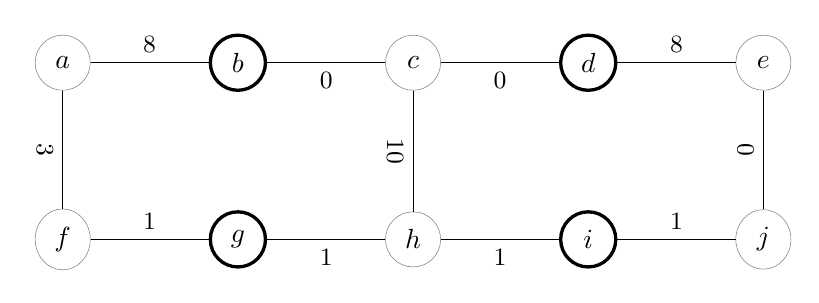
\begin{tikzpicture}[
normnode/.style={ellipse, draw=gray, very thin, minimum size=7mm},
prioritynode/.style={ellipse, draw=black, very thick, minimum size=7mm},
node distance=1.5cm and 1.5cm
]

%Nodes
\node[normnode] (a) {$a$};
\node[prioritynode] (b) [right=of a] {$b$};
\node[normnode] (c) [right=of b] {$c$};
\node[prioritynode] (d) [right=of c] {$d$};
\node[normnode] (e) [right=of d] {$e$};
\node[normnode] (f) [below=of a] {$f$};
\node[prioritynode] (g) [right=of f] {$g$};
\node[normnode] (h) [right=of g] {$h$};
\node[prioritynode] (i) [right=of h] {$i$};
\node[normnode] (j) [right=of i] {$j$};

\foreach \i/\j/\txt/\p in {% start node/end node/text/position
      a/b/{8}/above,
      b/c/{0}/below,
      c/d/{0}/below,
      d/e/{8}/above,
      a/f/{3}/below,
      c/h/{10}/below,
      e/j/{0}/below,
      f/g/{1}/above,
      g/h/{1}/below,
      h/i/{1}/below,
      i/j/{1}/above}
       \draw (\i) -- node[sloped,font=\small,\p] {\txt} (\j);
\end{tikzpicture}
\end{center}
The priority set $P=\{b,d,g,i\}$ and are drawn with darker circles.
Since $b$ and $d$ are already connected by undamaged roads, it'd
be tempting to fix the bridge $(c,h)$ and connect $(g,h)$ and $(h,i)$,
for a total cost of $0+0+10+1+1=12$.
However, you can do better by using the edges in $R=\{(b,c),(c,d),(d,e),(e,j),(i,j), (h,i), (g,h)\}$, which have a total cost of $0+0+8+0+1+1+1=11$.

Formally, we define the Restoring Transportation Network (RTN) problem
as follows:
\begin{quote}
Given a graph $G=(V,E)$,
a subset $P\subseteq V$,
a nonnegative cost $c(e)$ for each $e\in E$,
and a nonnegative budget $b$,
does there exist a subset of the edges $R\subseteq E$ that connects
all the vertices in $P$, the sum of whose costs is less than or equal
to $b$, i.e., $\sum_{r\in R} c(r) \le b$.
\end{quote}
Our goal in this question is to prove that RTN is NP-complete.

\begin{enumerate}
\item (3 marks)
Remember that a problem being NP-complete means both that it's in NP
and that it's NP-hard.  Therefore, any proof of NP-completeness has
two completely separate parts.  First, prove that RTN is in NP.

\begin{soln}
To show RTN is in NP, we will provide a verification algorithm. This will take in $G={V,E}$, $P$, $b$, and $R$.

We will simply ensure that the total sum of the edges in $R$ is less than or equal to $b$, and that this subset of edges connects all vertices in $P$, which can be done through a simple traversal using only the edges in $R$. If all of those are true, then this is a yes\_instance, otherwise it is a no\_instance. Every step is going to be polynomial time.


\end{soln}
\newpage
\item (3 marks)
The rest of an NP-completeness proof is to show that the problem is
NP-hard, by reducing a known NP-hard problem to it.
For this problem, you must do a reduction from the 3-Dimensional Matching
(3DM) problem.  (See Section~8.6 in the textbook, or the Wikipedia page
for ``3-dimensional matching''.)
For this part of the question, explain your reduction and why it runs
in polynomial time.  (You don't have to prove it correct yet; that comes
next!)

\textbf{Important Restriction (and Hint):}
To make this problem easier to mark, we \textbf{require} that
if your 3DM instance has $n$ elements in each of the sets $X$, $Y$, and $Z$,
and the size of the set of triples $|T|$ is $t$, then the RTN instance
you generate \textbf{must not have more than $3n+t+10$ vertices.}
(Our reduction uses exactly $3n+t+1$ vertices, but we allow you a few more
in case you think you need them.)  This is a restriction on you, but it's
also a hint in that it prevents you from doing anything too crazy, and
also gives some hints about what the graph might look like.

\begin{soln}
\includegraphics[width=400px]{new_reduction_3dm_to_rtn_3.png}

Above is a visual demonstration of the reduction, which I will now explain!

The reduction takes in the inputs to 3DM, which are the sets $X,Y,Z$ which each have size $n$, and the triplets set $T$, which has size $t$. We will refer to the 3DM instance as $I_3$. We will also define an instance of RTN as the graph $G=(V,E)$, the priority nodes $P\subseteq V$, the cost per edge $c(e \in E)$, and budget $b$, with the aim of selecting $R \subseteq E$ to connect up all nodes in $P$. The RTN instance will be called $I_R$. Here is the reduction:

Step 1: For each element of the sets $X, Y, Z$, create nodes for them, each node will be assigned labels based on which set they came from, so X nodes will be labelled $x_1,x_2,...,x_{n-1},x_n$, Y nodes $y_1,y_2,...,y_{n-1},y_n$, and Z nodes $z_1,z_2,...,z_{n-1},z_n$. Then, we also want to create nodes to represent the $t$ triples, and they will be labelled $T_1, T_2,...,T_{t-1},T_t$. This is in $\Theta(n + t)$.

Step 2: For each triple in T, create an edge between each element inside it and the triple node, i.e. for a triple $T_i = \{x_j, y_k, z_l\}$, create edges $(T_i, x_j), (T_i,  y_k), (T_i, z_l)$, and give each one of these an edge weight of 1. This is in $\Theta(t)$.

Step 3: Create a 'head' node, and create an edge $(head, T_i)$ for each T node with an edge weight of 0. This is in $\Theta(t)$.

Step 4: Add the $X, Y, Z$ nodes and the head node to the set $P$.  This is in $\Theta(n)$.

Step 5: Set $b=3n$.  This is in $\Theta(1)$.

We have now reduced $I_3$ to $I_R$ in polynomial time!
\end{soln}

\item (3 marks)
To prove your reduction correct, you must prove that
the answer to your RTN instance is ``yes'' if and only if
the answer to the 3DM instance is ``yes''.  For this part of the question,
prove one direction of this if-and-only-if.  In particular, prove
that if the answer to the 3DM instance is ``yes'', then the
answer to the RTN instance you reduce it to is also ``yes''.

\begin{soln}
Since there is a yes\_instance of $I_3$, that means there is a grouping of pairs in $T$ that matches up every element from $X,Y,Z$. Let's call this grouping of triplets U (for groUping of course). 

A good solution for $I_R$ is one where the sum of all weights in $R$ is less than or equal to 3n. 

For this grouping U, for each triplet $u \in U$, we will add all corresponding edges from that triplet node $T_u$ to the $X,Y,Z$ nodes it is connected to to the set R. We will also need to have to connect each triplet node $T_u$ to the head. That's it for the edge selection! 

The total number of these triplets in P is n, since in this perfect matching every node appears in only one match, and there are n nodes per 'dimension' of the triplet. Since each triplet node has 3 'children' (with children being defined as one X node, one Y node, and one Z node), there will be in total 3n edges between all T nodes and the children in the set R. Finally, to connect the final head node, we add no cost, so the final weight of our graph is $3n$. This number is less than or equal to the b we define, so it is valid!!!!

It is important to explain the weights more. We gave the nodes to the children a weight of 1, which enforces the fact that we will not be having more than one edge coming out of any child node, since any extra edge we add to R will increase the weight above 3n, which is greater than b. The 0 weight edges from the head ensure that the entire graph is connected together, with no penalties.

All this means that if $I_3$ is a yes\_instance, $I_R$ will be a yes\_instance.
\end{soln}

\item (3 marks)
Now, to complete the proof, you must prove the other direction of the
if-and-only-if:
prove
that if the answer to the RTN instance is ``yes'', then the
answer to the original 3DM instance is also ``yes''.

\begin{soln}
Since the question assumes a yes\_instance of $I_R$, that means that there is a path between all nodes in P (the shaded nodes) that sum to a weight less than or equal to b. What this means in our graph is that each child node (since every child node must be connected since it is in P) will take one path up to 1 T node, as if it had more than one edge connected to it in R we would end up with a resulting total weight above 3n, which cannot be allowed since we know from assumption this is a yes\_instance. This means that each child node from $X, Y, Z$ is connected to exactly one T node. This means that for every T node, it has 3 children, which corresponds to a triplet. Since every node in $X,Y,Z$ is connected to some T node, each element of $X,Y,Z$ is effectively in a triplet, meaning there is a way to group the three sets together through T, meaning that if $I_R$ was a yes\_instance, $I_3$ will also be a yes\_instance. Since both sides of the iff statement are true, RTN is NP-complete.
\end{soln}

\end{enumerate}

\end{document}

